\documentclass[10pt]{beamer}
% \setbeamercovered{transparent}
\beamerdefaultoverlayspecification{<+(1)-| alert@+(1)>}
\usetheme{Boadilla}
\usecolortheme{seahorse}
\usefonttheme{structurebold}
\usepackage{multicol}
\usepackage{graphicx}
\usepackage{tikz}
\usepackage{calc}
\usetikzlibrary{calc}
\usepackage{fp}
\usepackage{listings} % Pacote para destacar código fonte
\usepackage{amsmath} 
\usepackage{amssymb} 
\usepackage{helvet}
\usepackage{xcolor}
\usepackage{pgfplots}
\usepackage{array}
\usepackage{arydshln}
\usepackage{enumitem}
\pgfplotsset{compat=1.18}
\setlist[itemize]{label=\textbullet}

\lstset{
  language=C++,
  basicstyle=\small\ttfamily,
  numbers=left, 
  numberstyle=\tiny, 
  stepnumber=1, 
  numbersep=-30pt, 
}

\newcommand{\codecppNoTitle}[2][0.6]{
  \centering
  \begin{minipage}{#1\textwidth}
    %Referencia: https://ctan.dcc.uchile.cl/macros/latex/contrib/listings/listings.pdf
    \lstset{
      language=C++,
      numbers=left,
      numberstyle=\tiny,
      stepnumber=1,
      numbersep=5pt,
      showstringspaces = false,
      frame=shadowbox,
      commentstyle=\color{commentgreen},
      keywordstyle=\color{eminence},
      stringstyle=\color{red},
      backgroundcolor=\color{black!3},
      keywordstyle=\color{blue},
      rulesepcolor=\color{black!5},
      basicstyle=\small\ttfamily, % basic font setting
      emph={int,char,double,float,unsigned,void,bool},
      emphstyle={\color{blue}}
    }
    \lstinputlisting{#2}
  \end{minipage}}


% Definindo as cores para as palavras reservadas
\definecolor{keywordblue}{RGB}{0,0,255}
\definecolor{identifierblack}{RGB}{0,0,0}

\newcommand{\duascolunas}[2]{
  \begin{columns}
    \begin{column}{0.72\textwidth}
      #1
    \end{column}
    \begin{column}{0.28\textwidth}
		#2
	\end{column}
  \end{columns}
}

\title{Análise de Complexidade}
\subtitle{Parte 1}
\author{Prof. Kennedy Reurison Lopes}
\date{\today}

% Início do documento
\begin{document}

\frame{\titlepage}

\begin{frame}
    \frametitle{Introdução}

    \begin{itemize}
        \item Bem-vindos à apresentação sobre a complexidade de realizar uma tarefa!
        \item Hoje discutiremos exemplos de tarefas que podem ser complexas, mesmo não necessariamente estejam diretamente relacionados a algoritmos.
        \item Depois iremos direto ao assunto: Como identificar a complexidade em algoritmos.
    \end{itemize}
\end{frame}

\begin{frame}
    \frametitle{Ordenar uma pilha de livros}
    \begin{itemize}
        \item Imagine uma pilha desorganizada de livros.
        \item A tarefa é organizá-los em ordem alfabética.
        \item A complexidade aumenta à medida que a pilha de livros fica maior.
    \end{itemize}
\end{frame}

\begin{frame}
    \begin{figure}[htb]
        \centering
        
\includegraphics[width=0.9\textwidth]{wally.jpg}
        \label{fig:wally2}
    \end{figure}
\end{frame}

\begin{frame}
    \frametitle{Encontrar um item específico}
    \begin{itemize}\large
        \item Suponha que você precise encontrar um objeto específico em uma sala cheia de itens.
        \item Quanto mais desorganizada a sala e mais objetos houver, mais complexa será a tarefa de localizar o item desejado.
    \end{itemize}
\end{frame}

\begin{frame}
    \frametitle{Classificar uma coleção de fotos}

    \begin{itemize}
        \item Considere uma grande coleção de fotos digitais a ser classificada em categorias específicas.
        \item Quanto maior a coleção e mais complexas as categorias, mais complexa se torna a tarefa de análise e atribuição de tags apropriadas.
    \end{itemize}

    \begin{figure}[htb]
        \centering
        
\includegraphics[width=0.5\textwidth]{fotos.jpg}
        \caption{Exemplo de coleção de fotos a ser classificada.}
        \label{fig:fotos}
    \end{figure}
\end{frame}

\begin{frame}
    \frametitle{Resolver um quebra-cabeça complexo}

    \begin{itemize}
        \item Pegue um quebra-cabeça desafiador, como um cubo mágico ou um quebra-cabeça de encaixe complexo.
        \item À medida que o número de peças ou a complexidade do quebra-cabeça aumenta, encontrar a solução se torna mais difícil e requer mais tempo e esforço.
    \end{itemize}

    \begin{figure}[htb]
        \centering
        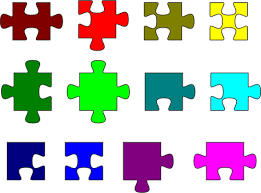
\includegraphics[width=0.4\textwidth]{quebracabeca}
        \label{fig:quebracabeca}
    \end{figure}
\end{frame}

\begin{frame}
    \frametitle{Planejar uma viagem com múltiplos destinos}
    \begin{itemize}
        \item Ao planejar uma viagem com vários destinos e restrições, como orçamento, tempo, logística, preferências pessoais, entre outros fatores, a complexidade aumenta.
        \item Quanto mais destinos e restrições envolvidos, mais complexo se torna o planejamento.
    \end{itemize}
\end{frame}

\begin{frame}[t]
    \frametitle{O que é um algoritmo?}
    \duascolunas{\begin{itemize}
            \item Um algoritmo é um conjunto \textbf{finito} de passos.
            \item Entretanto, a existência de um algoritmo não garante que possa ser resolvido.
            \item  Condições de tempo e memória devem ser avaliadas.
        \end{itemize}}{\begin{figure}[h]
            \centering
            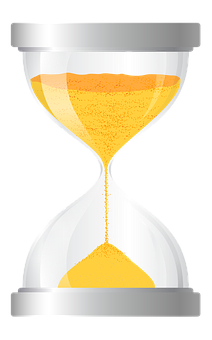
\includegraphics[width=1\textwidth]{Ampulheta}
        \end{figure}}
\end{frame}

\begin{frame}
    \frametitle{Recursos valiosos}
    \begin{itemize}
        \item Algoritmos demandam tempo de execução e recursos:
              \begin{itemize}
                  \item Memória
                  \item Espaço em disco
                  \item Dispositivos externos
                  \item Banda de rede
                  \item \ldots
              \end{itemize}
        \item Um bom programador deve ter o atributo de \textbf{poupar} tempo e recursos.
        \item A principal desempenho avaliado é a \emph{economia} do tempo necessário para o cálculo dos algoritmos.
    \end{itemize}
\end{frame}

\newcommand{\randomGrid}[1]{%
    \begin{tikzpicture}[scale=1]
        \def\gridSize{#1}
        \foreach \x in {1,...,\gridSize} {
                \foreach \y in {1,...,\gridSize} {
                        \pgfmathsetmacro{\randomColor}{rnd}
                        \pgfmathsetmacro{\randomNumber}{int(random(1,1000))}
                        \fill[red!20] (\x-1,\y-1) rectangle (\x,\y);
                        \node at (\x-0.5,\y-0.5) {\randomNumber};
                    }
            }
        \draw[step=1cm, fill=blue] (0,0) grid (\gridSize,\gridSize);
    \end{tikzpicture}%
}

\begin{frame}\frametitle{Quanto tempo preciso para organizar este grid?}
    \begin{center}
        \randomGrid{2}
    \end{center}
\end{frame}

\begin{frame}
    \frametitle{Quanto tempo preciso para organizar este grid?}
    \begin{center}
        \randomGrid{3}
    \end{center}
\end{frame}

\begin{frame}
    \frametitle{Quanto tempo preciso para organizar este grid?}
    \begin{center}
        \randomGrid{4}
    \end{center}
\end{frame}

\begin{frame}
    \frametitle{Quanto tempo preciso para organizar este grid?}
    \begin{center}
        \randomGrid{5}
    \end{center}
\end{frame}

\newcommand{\figuraRegular}[2]{%
    \begin{center}
        \begin{tikzpicture}
            \pgfmathsetmacro{\radius}{#2} % Raio da figura regular
            \pgfmathsetmacro{\angle}{360/#1} % Ângulo entre os lados da figura regular
            \pgfmathsetmacro{\apothem}{\radius*cos(\angle/2)} % Apótema da figura regular

            % Desenhar os vértices da figura regular
            \foreach \i in {1,...,#1} {
                    \pgfmathsetmacro{\x}{\radius*cos(\i*\angle)}
                    \pgfmathsetmacro{\y}{\radius*sin(\i*\angle)}
                    \coordinate (v\i) at (\x,\y);
                }

            % Desenhar a figura regular
            \draw (v1)
            \foreach \i in {2,...,#1} {
                    -- (v\i)
                } -- cycle;

            % Desenhar o apótema
            \draw[dashed] (0,0) -- (v1) node[midway, above] {};
            \draw[dashed] (0,0) -- (v2) node[midway, above] {};

            \node[anchor=west, xshift=1cm, text width=8cm] at (0.5,0) {
                \pgfmathsetmacro{\alfa}{(180 - (360/#1))/2}
                \pgfmathsetmacro{\alfaB}{tan(\alfa)}
                \pgfmathsetmacro{\Atotal}{#1*2*\alfaB/2}
                \pgfmathsetmacro{\diag}{2*sqrt(1+\alfaB*\alfaB)}

                \pgfmathsetmacro{\pAlfa}{round(100*\alfa)/100}
                \pgfmathsetmacro{\pAlfaB}{round(100*\alfaB)/100}
                \pgfmathsetmacro{\pTotal}{round(100*\Atotal)/100}
                \pgfmathsetmacro{\PT}{2*#1}
                \pgfmathsetmacro{\razao}{\PT/\diag}

                \begin{align*}
                    2*\alpha   & = \left(180 - \frac{360}{#1}\right) \rightarrow \alpha   = \pAlfa ^o \\
                    tg(\alpha) & = \frac{h}{L/2}          \rightarrow h                 = \pAlfaB     \\
                    P_T        & = #1L      = \PT                                                     \\
                    D          & = 2\sqrt{1+h^2}= \diag                                               \\
                    \pi        & \approx P_T/D = \razao
                \end{align*}
            };
        \end{tikzpicture}
    \end{center}
}

\newcommand{\slidefiguraRegular}[2]{
    \begin{frame}
        \frametitle{Cálculo do $\pi$ (Alg. 1)}
        \framesubtitle{#2 lados  ($L=2$)}
        \figuraRegular{#2}{#1}
    \end{frame}
}

\foreach \i in {3,...,20} {
        \slidefiguraRegular{2}{\i}
    }

\begin{frame}
    \begin{center}
        \begin{tikzpicture}
            \frametitle{Cálculo do $\pi$ (Alg. 1)}
            \draw[fill=none](0,0) circle (2.0);
            \draw (0,0) -- (2,0) node[midway, yshift=10] {R};
            \node[anchor=west, xshift=1cm, text width=6cm] at (2,0.5) {
                $$\lim_{n\rightarrow\infty}\left(\frac{P_T}{D}\right) = \left(\frac{2 \pi R}{2R}\right)= \pi$$
            };
        \end{tikzpicture}
    \end{center}
\end{frame}


\newcounter{bluePointsCounter}
\newcommand{\circuloEQuadrado}[1]{
    \setcounter{bluePointsCounter}{0}
    \begin{tikzpicture}
        \draw (0,0) rectangle (4,4);
        \draw (2,2) circle [radius=2cm];
        \fill (2,2) circle [radius=0.5pt];
        \foreach \i in {1,...,#1}
            {
                \pgfmathsetmacro{\x}{random()*4}
                \pgfmathsetmacro{\y}{random()*4}

                % Verifica se o ponto está dentro do círculo
                \pgfmathparse{(\x-2)^2 + (\y-2)^2 <= 2^2 ? int(1) : int(0)}
                \ifnum\pgfmathresult=1
                    \fill[blue] (\x,\y) circle [radius=1pt];
                    \stepcounter{bluePointsCounter} % Incrementa o contador
                \else
                    \fill[red] (\x,\y) circle [radius=1pt];
                \fi
            }

        % Exibe o valor do contador
        \def\azul{\thebluePointsCounter}
        \node[anchor=west] at (6,3.5) {Pontos Azuis(A): \thebluePointsCounter};
        \pgfmathsetmacro{\vermelhos}{#1 - \thebluePointsCounter};
        \node[anchor=west] at (6,2.5) {Pontos Vermelhos(V): \vermelhos};
        \node[anchor=west] at (6,1.5) {Totais(T): #1};
        \pgfmathsetmacro{\razao}{4*\azul/#1};
        \node[anchor=west] at (6,0.5) {4*Razão (A/T): \razao};
        \draw[|-|] (0,-0.5) -- node[below] {$L=4$} (4,-0.5);
        \draw[|-|] (2,2) -- node[below] {$R=2$} ++(2,0);
    \end{tikzpicture}
}
\newcommand{\calcpi}[1]{
    \begin{frame}
        \frametitle{Cálculo do $\pi$ (Alg. 2)}
        \circuloEQuadrado{#1}
    \end{frame}
}
\foreach \i in {10,20,...,200} {
        \calcpi{\i}
    }

\begin{frame}[t]
    \frametitle{Cálculo de $\pi$ (Alg. 2)}
    \circuloEQuadrado{1000}

    Quando os pontos tendem ao infinito:
    \begin{align*}
        \lim_{N\rightarrow\infty} A/T = \frac{A_c}{A_q} = \frac{\pi R^2}{(2R)^2} = \frac{\pi}{4}
    \end{align*}

\end{frame}

\end{document}